\section{Gestionnaire des inscriptions}

Cette section décrit les actions principales de la page gestionnaire des inscriptions. Cette page n'est accessible qu'aux membre du staff avec la permission de gérer les inscriptions (voir la section "Gestionnaire des permissions").\newline

Cette page de gestionnaire des inscriptions permet de gérer les frais d'inscription au tournoi, la date du début de l'événement Le Charles de Lorraine, et un panneau de configuration des extras.\newline

Cette page est divisée en 2 parties : le module du haut permet de gérer les frais d'inscription et la date du tournoi, tandis que le module du bas permet de gérer les extras.

\begin{figure}[H]
\centering
\includegraphics[scale=0.15]{user_images/staff/GererInscription/001.jpg}
\caption{Gestionnaire des inscriptions}
\end{figure}

\subsection{Modifier les frais d'inscription et la date du tournoi}

Pour modifier les frais d'inscription et la date du tournoi, il suffit de modifier les champs du module du haut "Tournoi".

\begin{figure}[H]
\centering
\includegraphics[scale=0.15]{user_images/staff/GererInscription/ModifierFraisInscription/001.jpg}
\caption{Modifier les frais d'inscription, étape 1}
\end{figure}

En modifiant les frais d'inscription (ici à 15,00), et la date du début du tournoi (ici au 10 septembre 2015), cliquez ensuite sur le bouton "Editer" du module du haut pour valider l'édition des frais d'inscription et de la date du tournoi.

\begin{figure}[H]
\centering
\includegraphics[scale=0.15]{user_images/staff/GererInscription/ModifierDate/001.jpg}
\caption{Modifier la date du tournoi, étape 2}
\end{figure}

L'historique des modifications des inscriptions, en bas de la page du gestionnaire des inscriptions, contient une nouvelle entrée de ces modifications sur les frais d'inscription et sur la date de début du tournoi.

MISSING FIGURE!

La date du début du tournoi a bien été édité. Cette modification est visible sur la page d'accueil du site web.

\begin{figure}[H]
\centering
\includegraphics[scale=0.15]{user_images/staff/GererInscription/ModifierDate/002.jpg}
\caption{Modifier la date du tournoi, étape 3}
\end{figure}

\subsection{Ajouter un extra}

Cette sous-section explique comment ajouter un nouvel extra lors de l'inscription à un tournoi. La partie extra correspond au module du bas de la page "Gestionnaire des inscriptions".\newline

En bas à gauche, il y a une liste des extras. Pour chacun des extra, un nombre en rouge indique le nombre de joueurs inscrits qui ont sélectionné cet extra lors de leur inscription.\newline

Pour ajouter un extra, cliquez sur le lien "Ajouter un extra" sous la liste des extras. Ensuite, remplissez les champs du nouvel extra à droite : le nom, le prix, et un commentaire de l'extra.\newline

Dès que les champs du nouvel extra sont remplis, cliquez sur le bouton "Ajouter" pour confirmer l'ajout de ce nouvel extra.

\begin{figure}[H]
\centering
\includegraphics[scale=0.15]{user_images/staff/GererInscription/AjouterExtra/001.jpg}
\caption{Ajouter un extra, étape 1}
\end{figure}

Un message en vert, entre les deux modules, indique le bon ajout de cet extra à la liste des extras.

\begin{figure}[H]
\centering
\includegraphics[scale=0.15]{user_images/staff/GererInscription/AjouterExtra/002.jpg}
\caption{Ajouter un extra, étape 2}
\end{figure}

L'historique des modifications des extras, en bas de la page, confirme à nouveau l'ajout récente de l'extra.

MISSING FIGURE!

\subsection{Modifier un extra}

Cette sous-section décrit comment modifier un extra dans la liste des extras. Tout d'abord, sélectionnez l'extra à modifier dans la liste des extras à gauche (Ici "Cinéma"). Les informations de l'extra sélectionné sont insérées dans des champs éditables, à droite.

\begin{figure}[H]
\centering
\includegraphics[scale=0.15]{user_images/staff/GererInscription/EditerExtra/001.jpg}
\caption{Modifier un extra, étape 1}
\end{figure}

Pour modifier un extra, il suffit de modifier les champs de l'extra. Ici, nous avons simplement modifié le champ "Commentaires" de l'extra ("8 ans et +", au lieu de "10 ans et +"). Après modifications des champs, cliquez sur le bouton "Editer" en bas du module "Editer Cinéma".

\begin{figure}[H]
\centering
\includegraphics[scale=0.15]{user_images/staff/GererInscription/EditerExtra/002.jpg}
\caption{Modifier un extra, étape 2}
\end{figure}

Après avoir valider l'édition de l'extra, un message vert entre les 2 modules signale la bonne modification de l'extra.

\begin{figure}[H]
\centering
\includegraphics[scale=0.15]{user_images/staff/GererInscription/EditerExtra/003.jpg}
\caption{Modifier un extra, étape 3}
\end{figure}

En bas de la page "Gestionnaire des inscriptions", une nouvelle entrée de l'historique des inscriptions confirme à nouveau la modification récente de l'extra.

MISSING FIGURE!

\subsection{Supprimer un extra}

Cette sous-section explique comment supprimer un extra dans la liste des extras. Dans la liste des extras, cliquez sur l'extra à supprimer (ici Cinéma), et cliquez sur le bouton "Supprimer" dans le module "Editer Cinéma".

\begin{figure}[H]
\centering
\includegraphics[scale=0.15]{user_images/staff/GererInscription/SupprimerExtra/001.jpg}
\caption{Supprimer un extra, étape 1}
\end{figure}

Après avoir cliqué sur le bouton "Supprimer", une boîte de dialogue demande confirmation de l'utilisateur, puisque cette suppression est irréversible.

\begin{figure}[H]
\centering
\includegraphics[scale=0.15]{user_images/staff/GererInscription/SupprimerExtra/002.jpg}
\caption{Supprimer un extra, étape 2}
\end{figure}

Après confirmation de la suppression de l'extra de la part de l'utilisateur, un message vert signale la bonne suppresion de l'extra.

\begin{figure}[H]
\centering
\includegraphics[scale=0.15]{user_images/staff/GererInscription/SupprimerExtra/003.jpg}
\caption{Supprimer un extra, étape 3}
\end{figure}

En bas de la page "Gestionnaire des inscriptions", l'historique des modifications des inscriptions confirme, à nouveau, la suppression récente de l'extra.

MISSING FIGURE!

\subsection{Nettoyer la base de données pour l'année suivante}

Pour nettoyer la base de données pour l'année suivante, un membre du staff peut effectuer cette opération s'il a la permission de gérer les inscriptions.\newline

Cliquez sur le bouton "Nettoyer la base de données pour l'année suivante", en bas de la page.

\begin{figure}[H]
\centering
\includegraphics[scale=0.15]{user_images/staff/GererInscription/NettoyerBDD/001.jpg}
\caption{Nettoyage de la base de donnée pour l'année prochaine, étape 1}
\end{figure}

Étant donnée que l'action est irréversible et a des implications importantes sur la base de données, une boîte de dialogue avec un avertissement ATTENTION, indique à l'utilisateur de confirmer son action.

\begin{figure}[H]
\centering
\includegraphics[scale=0.15]{user_images/staff/GererInscription/NettoyerBDD/002.jpg}
\caption{Nettoyage de la base de donnée pour l'année prochaine, étape 2}
\end{figure}

Après avoir confirmé le nettoyage de la base de donnée pour l'année suivante, la base de donnée subit plusieurs changements pour se préparer pour l'année suivante. En particulier, toutes les paires sont retirés, les anciens utilisateurs et terrains sont indiqués comment vétérans, et tous les tournois sont vidés, comme indiqué sur l'image ci-dessous.

\begin{figure}[H]
\centering
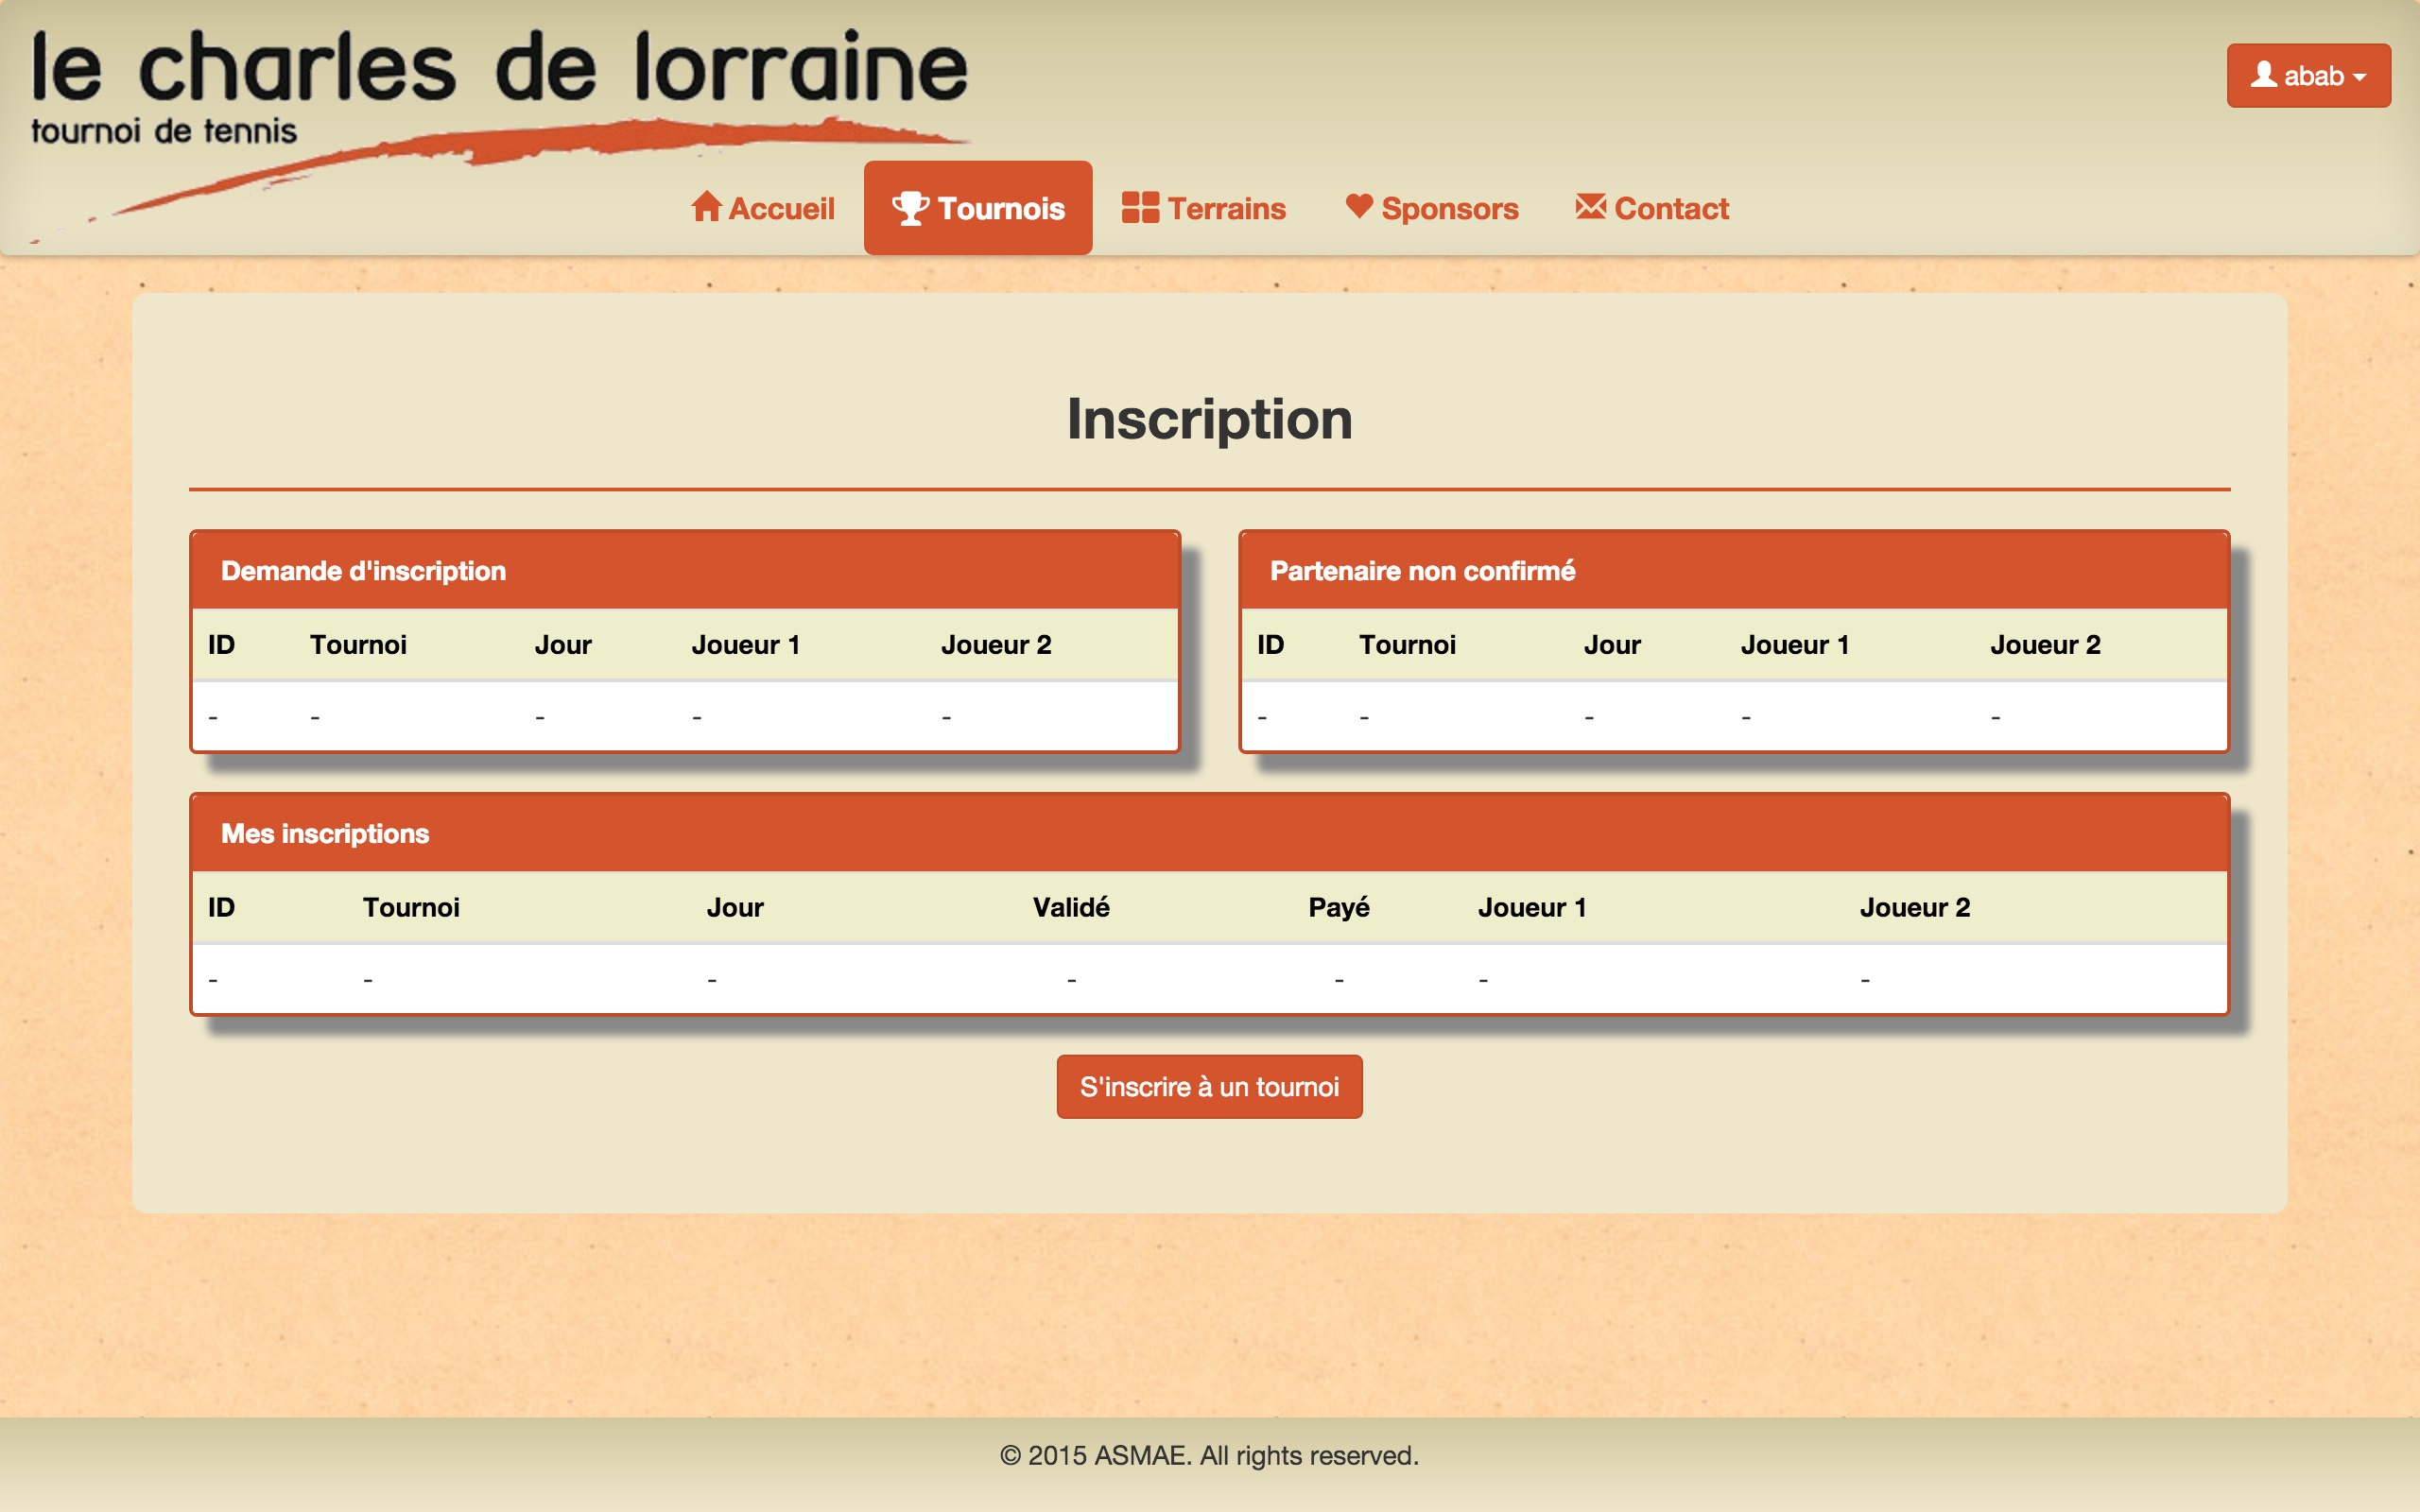
\includegraphics[scale=0.15]{user_images/staff/GererInscription/NettoyerBDD/005.jpg}
\caption{Nettoyage de la base de donnée pour l'année prochaine, état des tournois}
\end{figure}
